\documentclass[11pt]{article}
\usepackage[textwidth=18.0cm, textheight=23.0cm, top=2.0cm]{geometry}
\usepackage{pst-all}
\usepackage{amssymb}
\usepackage{tikz}
\usepackage{underscore}\begin{document}
\pagestyle{empty}


ClassName: \underline{\textbf{Class_10.2bp-31}}
\par
BinSize: \underline{\textbf{100 × 100}}
\par
ReduceSize: \underline{\textbf{100 × 100}}
\par
TypeNum: \underline{\textbf{80}}
\par
Num: \underline{\textbf{80}}
\par
OutS: \underline{\textbf{110000}}
\par
InS: \underline{\textbf{97806}}
\par
Rate: \underline{\textbf{0.889}}
\par
UB: \underline{\textbf{11}}
\par
LB0: \underline{\textbf{10}}
\par
LB: \underline{\textbf{11}}
\par
LBWithCut: \underline{\textbf{11}}
\par
NodeCut: \underline{\textbf{0}}
\par
ExtendedNodeCnt: \underline{\textbf{1}}
\par
GenNodeCnt: \underline{\textbf{1}}
\par
PrimalNode: \underline{\textbf{0}}
\par
ColumnCount: \underline{\textbf{43}}
\par
TotalCutCount: \underline{\textbf{0}}
\par
RootCutCount: \underline{\textbf{0}}
\par
LPSolverCnt: \underline{\textbf{33}}
\par
PricingSolverCnt: \underline{\textbf{33}}
\par
BranchAndBoundNum: \underline{\textbf{1}}
\par
isOpt: \underline{\textbf{false}}
\par
TimeOnInitSolution: \underline{\textbf{600.000 s}}
\par
TimeOnPrimal: \underline{\textbf{0.000 s}}
\par
TimeOnPricing: \underline{\textbf{2999.646 s}}
\par
TimeOnRmp: \underline{\textbf{0.080 s}}
\par
TotalTime: \underline{\textbf{3600.007 s}}
\par
\newpage


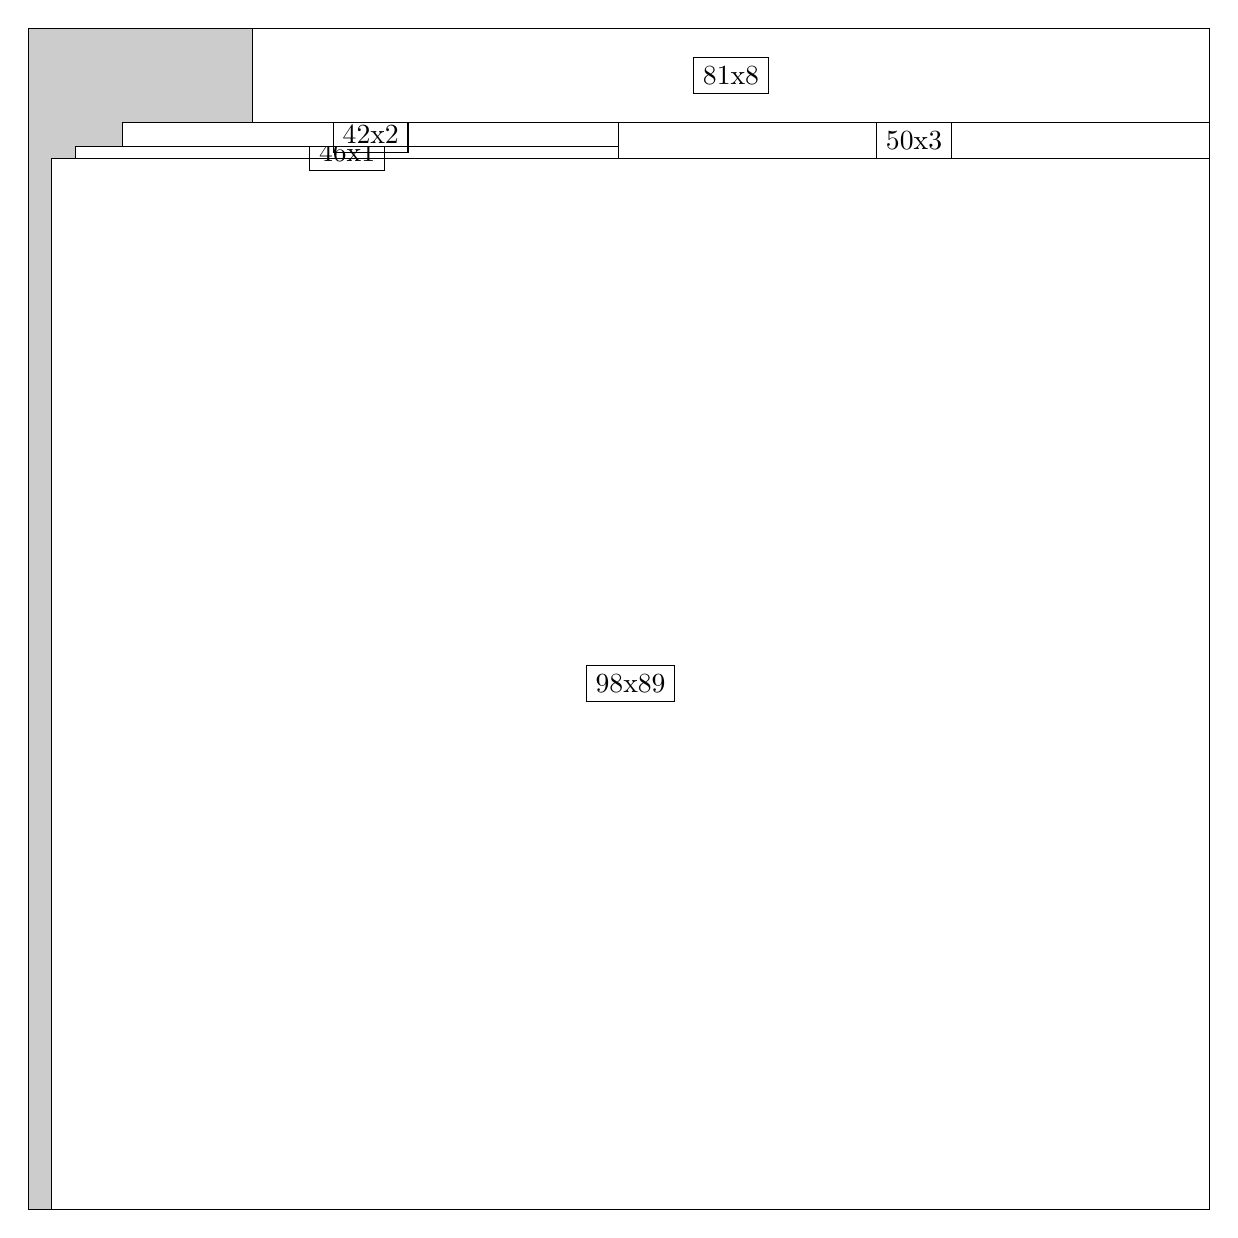
\begin{tikzpicture}[shorten >=1pt,scale=1.0,every node/.style={scale=1.0},->]
\tikzstyle{vertex}=[circle,fill=black!25,minimum size=14pt,inner sep=0pt]
\filldraw[fill=gray!40!white, draw=black] (0,0) rectangle (15.0,15.0);
\foreach \name/\x/\y/\w/\h in {98x89/0.3/0.0/14.7/13.35,50x3/7.5/13.35/7.5/0.44999999999999996,46x1/0.6/13.35/6.8999999999999995/0.15,42x2/1.2/13.5/6.3/0.3,81x8/2.85/13.799999999999999/12.15/1.2}
\filldraw[fill=white!40!white, draw=black] (\x,\y) rectangle node[draw] (\name) {\name} ++(\w,\h);
\end{tikzpicture}


w =98 , h =89 , x =2 , y =0 , v =8722
\par
w =50 , h =3 , x =50 , y =89 , v =150
\par
w =46 , h =1 , x =4 , y =89 , v =46
\par
w =42 , h =2 , x =8 , y =90 , v =84
\par
w =81 , h =8 , x =19 , y =92 , v =648
\par
\newpage


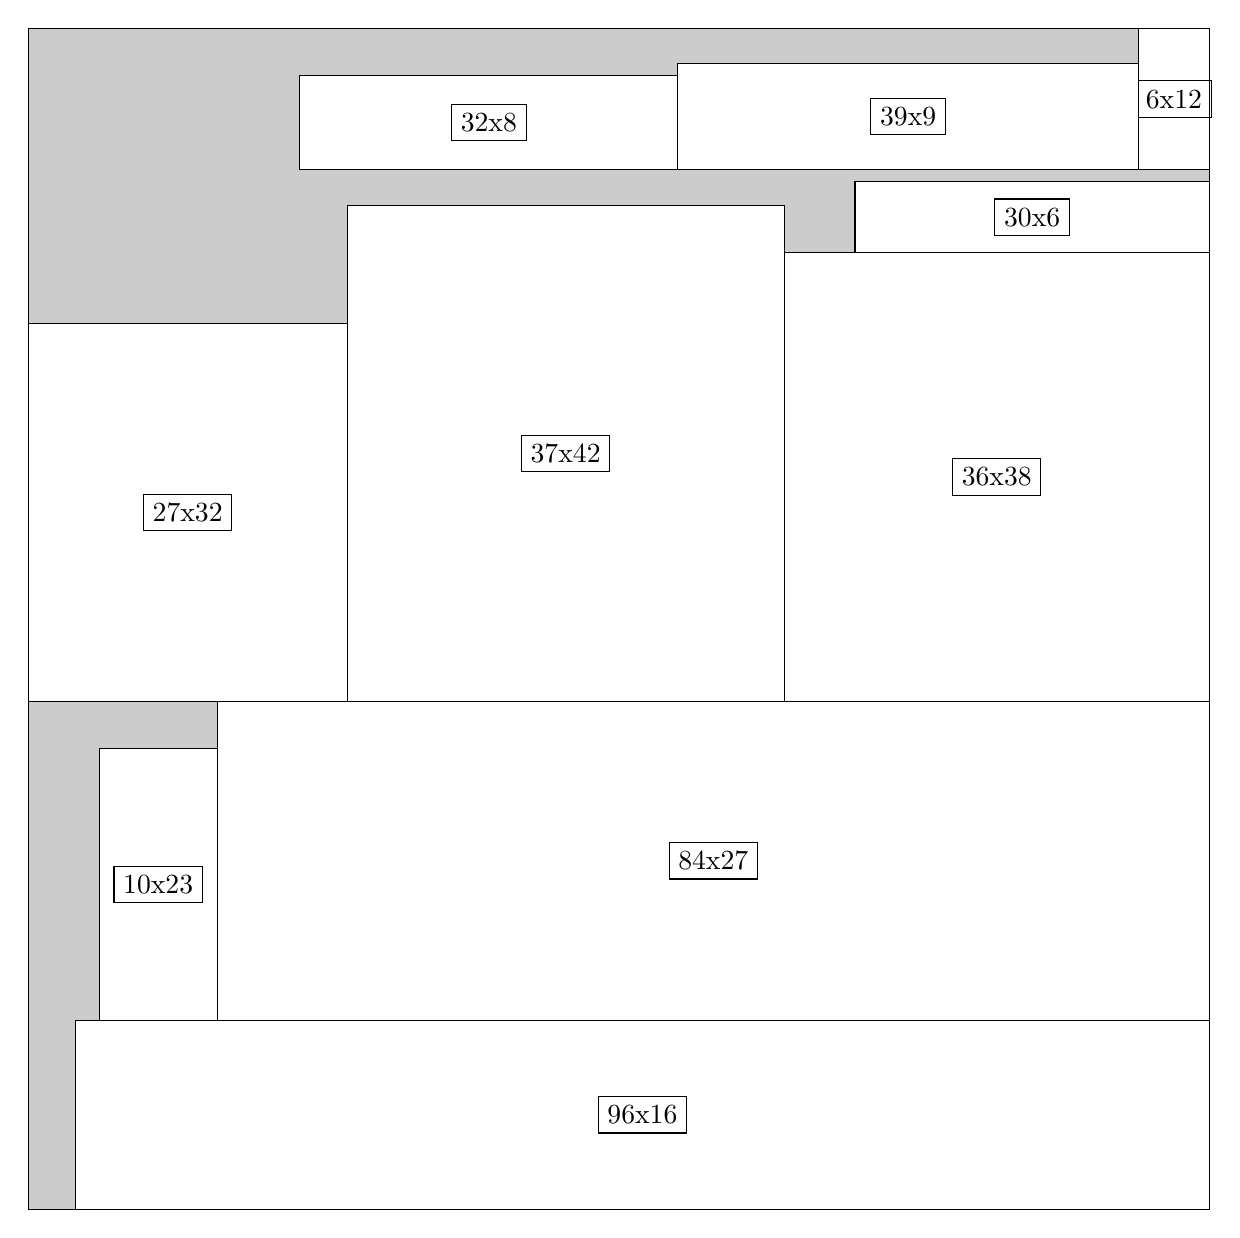
\begin{tikzpicture}[shorten >=1pt,scale=1.0,every node/.style={scale=1.0},->]
\tikzstyle{vertex}=[circle,fill=black!25,minimum size=14pt,inner sep=0pt]
\filldraw[fill=gray!40!white, draw=black] (0,0) rectangle (15.0,15.0);
\foreach \name/\x/\y/\w/\h in {96x16/0.6/0.0/14.399999999999999/2.4,84x27/2.4/2.4/12.6/4.05,10x23/0.8999999999999999/2.4/1.5/3.4499999999999997,36x38/9.6/6.45/5.3999999999999995/5.7,30x6/10.5/12.15/4.5/0.8999999999999999,37x42/4.05/6.45/5.55/6.3,27x32/0.0/6.45/4.05/4.8,6x12/14.1/13.2/0.8999999999999999/1.7999999999999998,39x9/8.25/13.2/5.85/1.3499999999999999,32x8/3.4499999999999997/13.2/4.8/1.2}
\filldraw[fill=white!40!white, draw=black] (\x,\y) rectangle node[draw] (\name) {\name} ++(\w,\h);
\end{tikzpicture}


w =96 , h =16 , x =4 , y =0 , v =1536
\par
w =84 , h =27 , x =16 , y =16 , v =2268
\par
w =10 , h =23 , x =6 , y =16 , v =230
\par
w =36 , h =38 , x =64 , y =43 , v =1368
\par
w =30 , h =6 , x =70 , y =81 , v =180
\par
w =37 , h =42 , x =27 , y =43 , v =1554
\par
w =27 , h =32 , x =0 , y =43 , v =864
\par
w =6 , h =12 , x =94 , y =88 , v =72
\par
w =39 , h =9 , x =55 , y =88 , v =351
\par
w =32 , h =8 , x =23 , y =88 , v =256
\par
\newpage


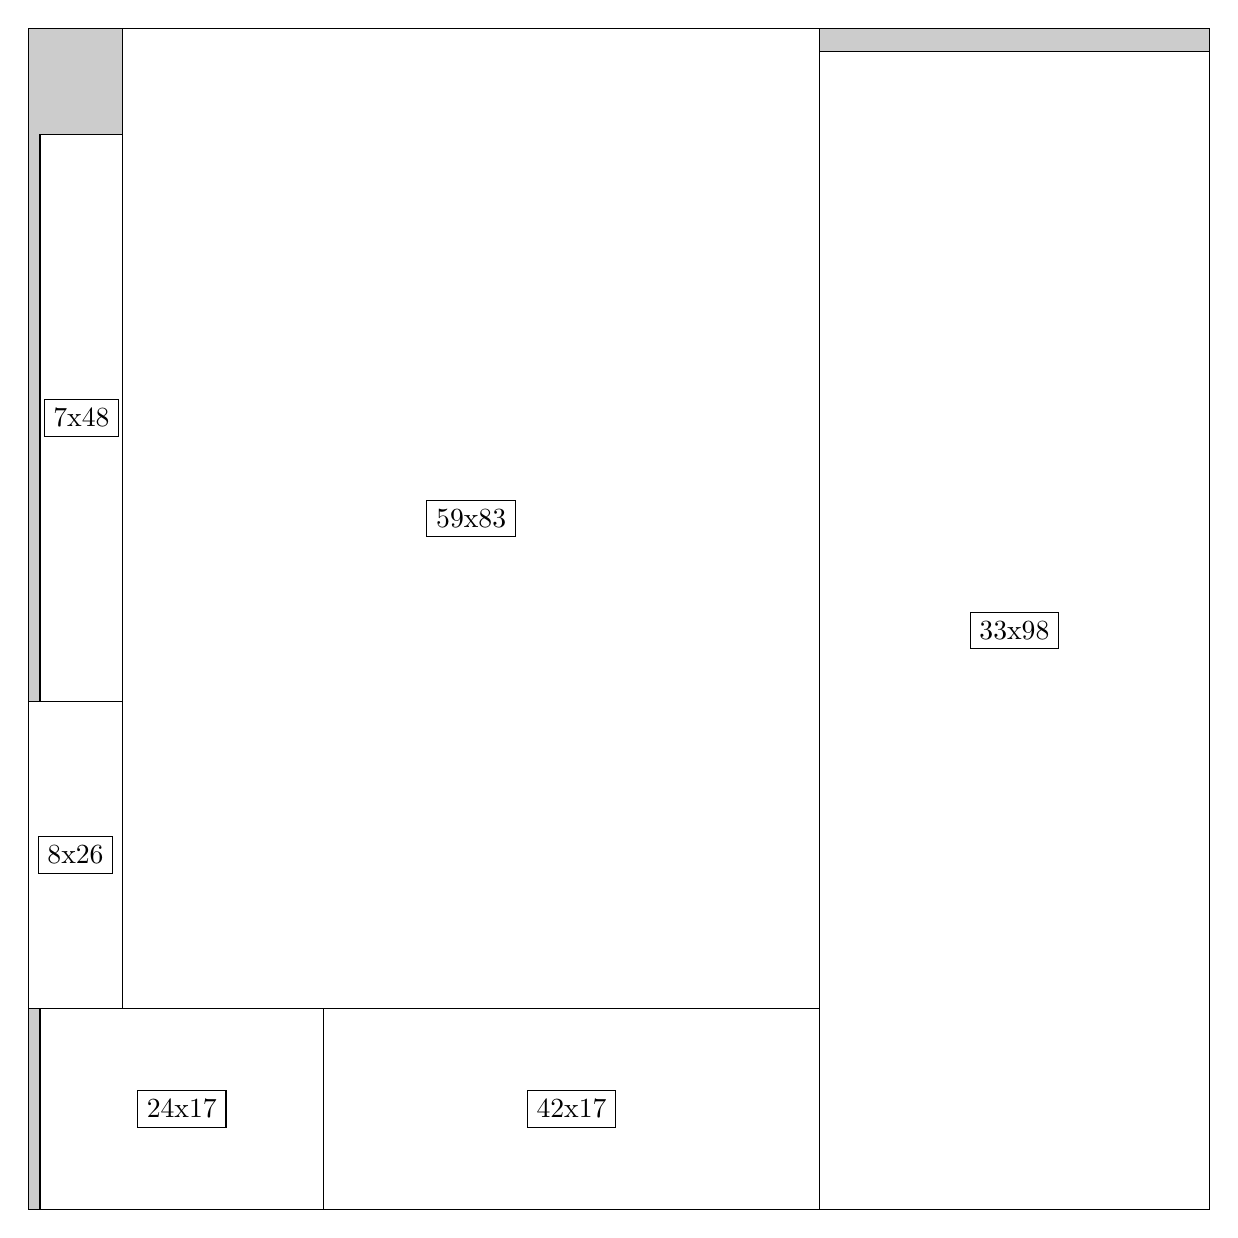
\begin{tikzpicture}[shorten >=1pt,scale=1.0,every node/.style={scale=1.0},->]
\tikzstyle{vertex}=[circle,fill=black!25,minimum size=14pt,inner sep=0pt]
\filldraw[fill=gray!40!white, draw=black] (0,0) rectangle (15.0,15.0);
\foreach \name/\x/\y/\w/\h in {33x98/10.049999999999999/0.0/4.95/14.7,42x17/3.75/0.0/6.3/2.55,24x17/0.15/0.0/3.5999999999999996/2.55,59x83/1.2/2.55/8.85/12.45,8x26/0.0/2.55/1.2/3.9,7x48/0.15/6.45/1.05/7.199999999999999}
\filldraw[fill=white!40!white, draw=black] (\x,\y) rectangle node[draw] (\name) {\name} ++(\w,\h);
\end{tikzpicture}


w =33 , h =98 , x =67 , y =0 , v =3234
\par
w =42 , h =17 , x =25 , y =0 , v =714
\par
w =24 , h =17 , x =1 , y =0 , v =408
\par
w =59 , h =83 , x =8 , y =17 , v =4897
\par
w =8 , h =26 , x =0 , y =17 , v =208
\par
w =7 , h =48 , x =1 , y =43 , v =336
\par
\newpage


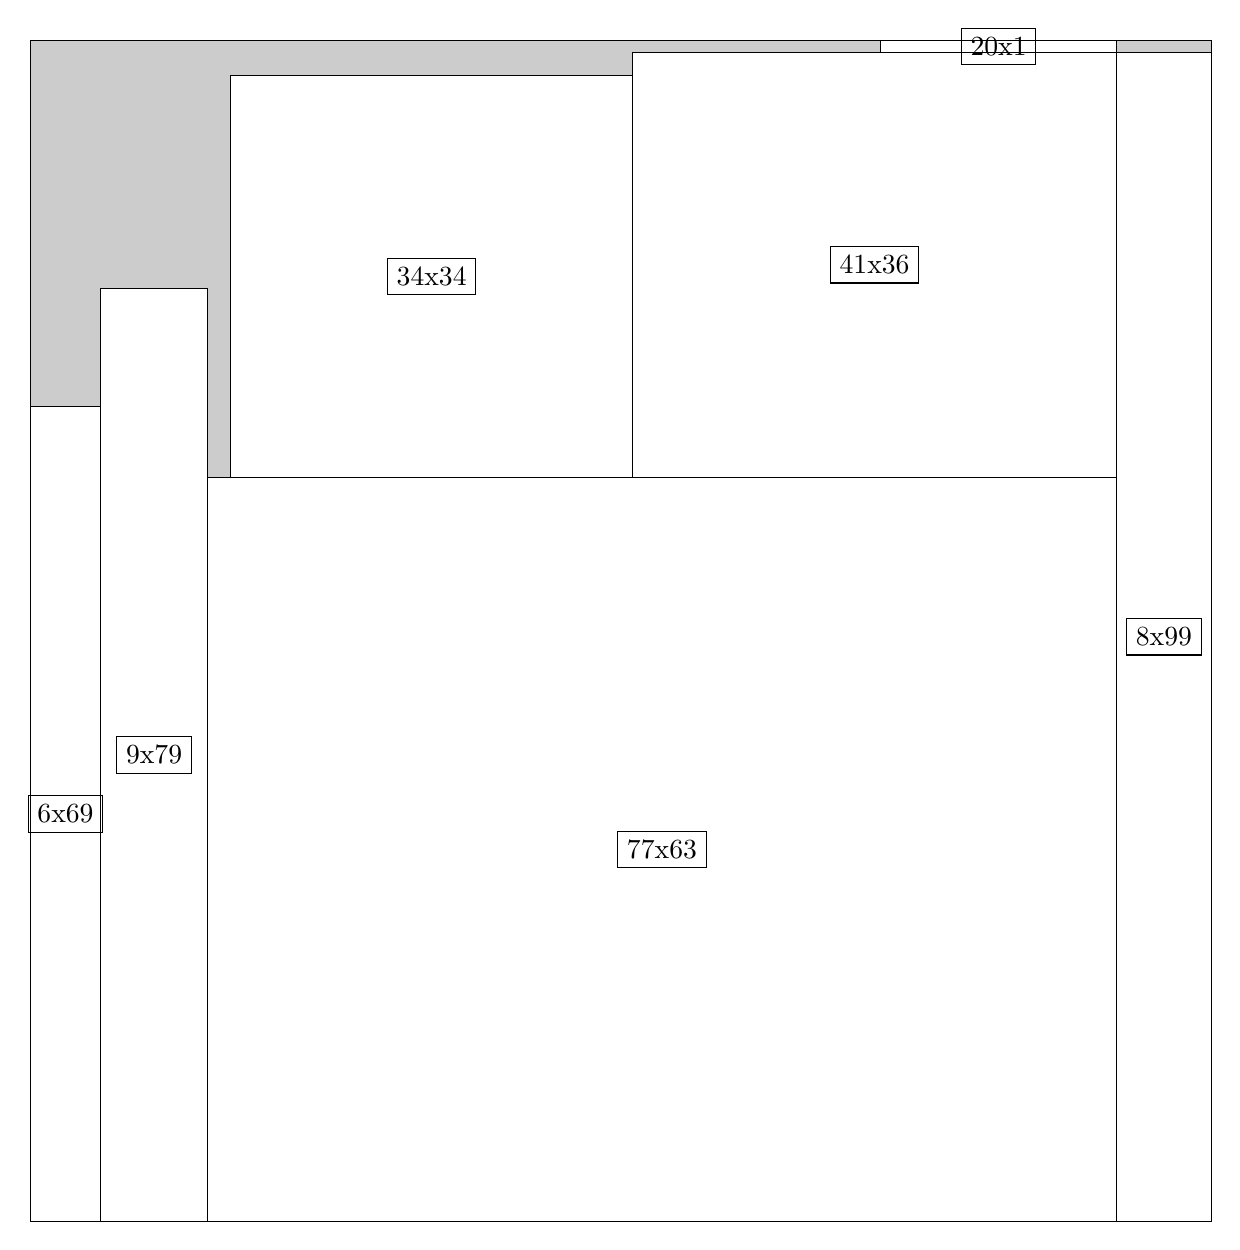
\begin{tikzpicture}[shorten >=1pt,scale=1.0,every node/.style={scale=1.0},->]
\tikzstyle{vertex}=[circle,fill=black!25,minimum size=14pt,inner sep=0pt]
\filldraw[fill=gray!40!white, draw=black] (0,0) rectangle (15.0,15.0);
\foreach \name/\x/\y/\w/\h in {8x99/13.799999999999999/0.0/1.2/14.85,77x63/2.25/0.0/11.549999999999999/9.45,41x36/7.6499999999999995/9.45/6.1499999999999995/5.3999999999999995,20x1/10.799999999999999/14.85/3.0/0.15,34x34/2.55/9.45/5.1/5.1,9x79/0.8999999999999999/0.0/1.3499999999999999/11.85,6x69/0.0/0.0/0.8999999999999999/10.35}
\filldraw[fill=white!40!white, draw=black] (\x,\y) rectangle node[draw] (\name) {\name} ++(\w,\h);
\end{tikzpicture}


w =8 , h =99 , x =92 , y =0 , v =792
\par
w =77 , h =63 , x =15 , y =0 , v =4851
\par
w =41 , h =36 , x =51 , y =63 , v =1476
\par
w =20 , h =1 , x =72 , y =99 , v =20
\par
w =34 , h =34 , x =17 , y =63 , v =1156
\par
w =9 , h =79 , x =6 , y =0 , v =711
\par
w =6 , h =69 , x =0 , y =0 , v =414
\par
\newpage


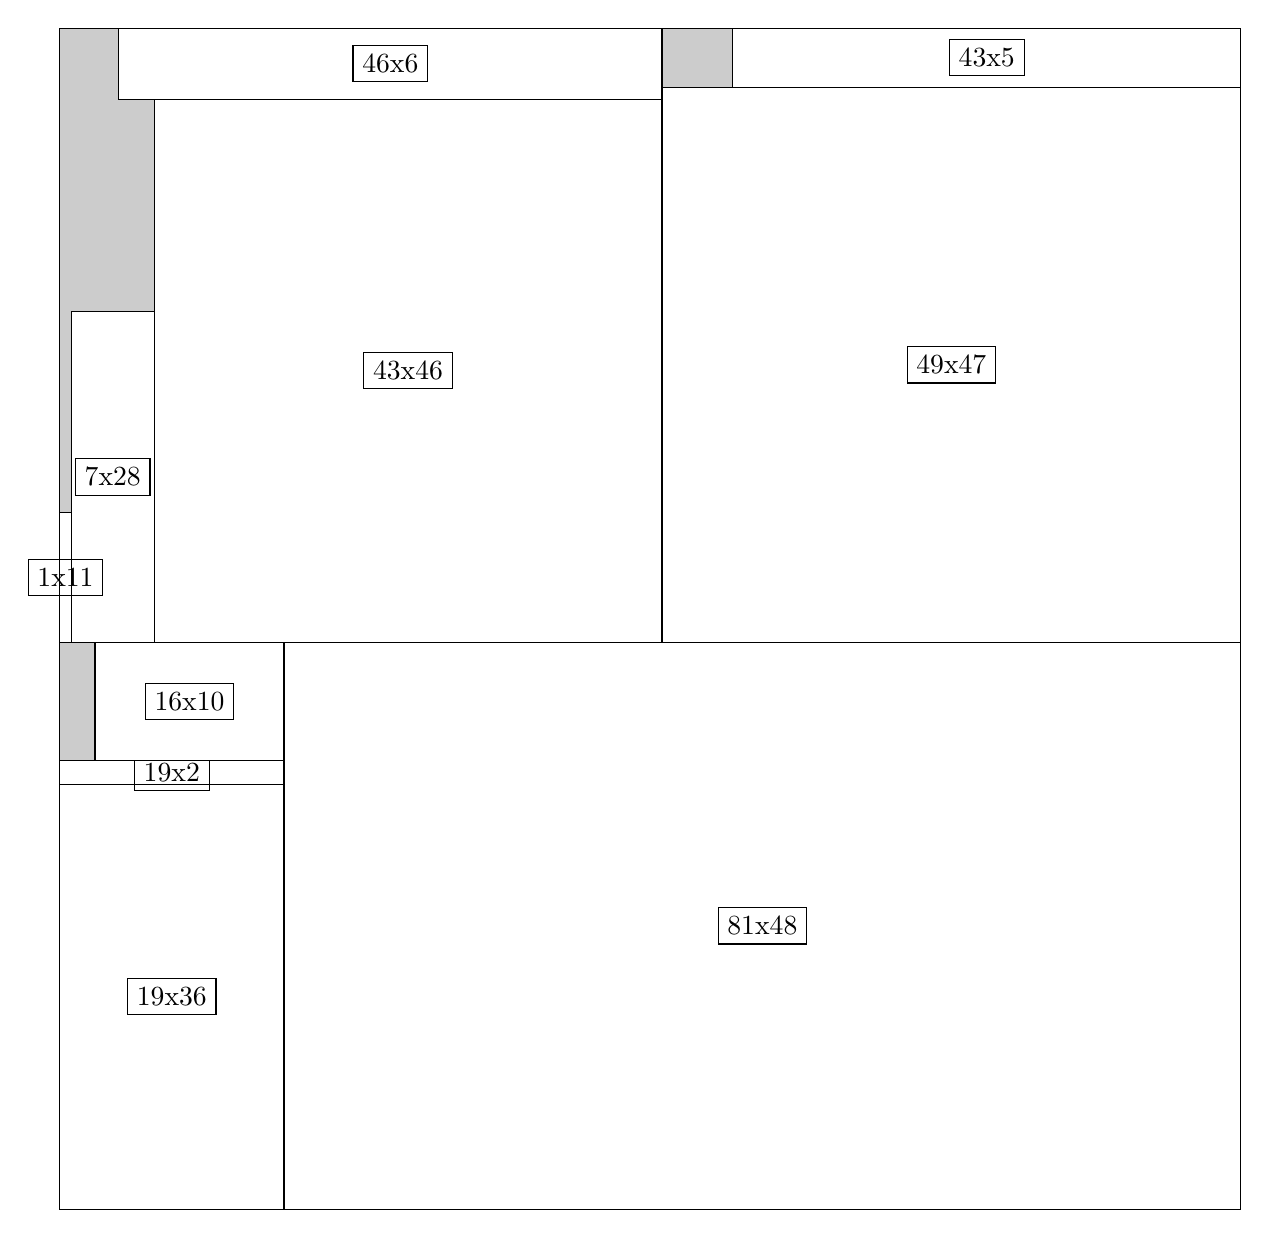
\begin{tikzpicture}[shorten >=1pt,scale=1.0,every node/.style={scale=1.0},->]
\tikzstyle{vertex}=[circle,fill=black!25,minimum size=14pt,inner sep=0pt]
\filldraw[fill=gray!40!white, draw=black] (0,0) rectangle (15.0,15.0);
\foreach \name/\x/\y/\w/\h in {81x48/2.85/0.0/12.15/7.199999999999999,19x36/0.0/0.0/2.85/5.3999999999999995,19x2/0.0/5.3999999999999995/2.85/0.3,16x10/0.44999999999999996/5.7/2.4/1.5,49x47/7.6499999999999995/7.199999999999999/7.35/7.05,43x5/8.549999999999999/14.25/6.45/0.75,43x46/1.2/7.199999999999999/6.45/6.8999999999999995,7x28/0.15/7.199999999999999/1.05/4.2,1x11/0.0/7.199999999999999/0.15/1.65,46x6/0.75/14.1/6.8999999999999995/0.8999999999999999}
\filldraw[fill=white!40!white, draw=black] (\x,\y) rectangle node[draw] (\name) {\name} ++(\w,\h);
\end{tikzpicture}


w =81 , h =48 , x =19 , y =0 , v =3888
\par
w =19 , h =36 , x =0 , y =0 , v =684
\par
w =19 , h =2 , x =0 , y =36 , v =38
\par
w =16 , h =10 , x =3 , y =38 , v =160
\par
w =49 , h =47 , x =51 , y =48 , v =2303
\par
w =43 , h =5 , x =57 , y =95 , v =215
\par
w =43 , h =46 , x =8 , y =48 , v =1978
\par
w =7 , h =28 , x =1 , y =48 , v =196
\par
w =1 , h =11 , x =0 , y =48 , v =11
\par
w =46 , h =6 , x =5 , y =94 , v =276
\par
\newpage


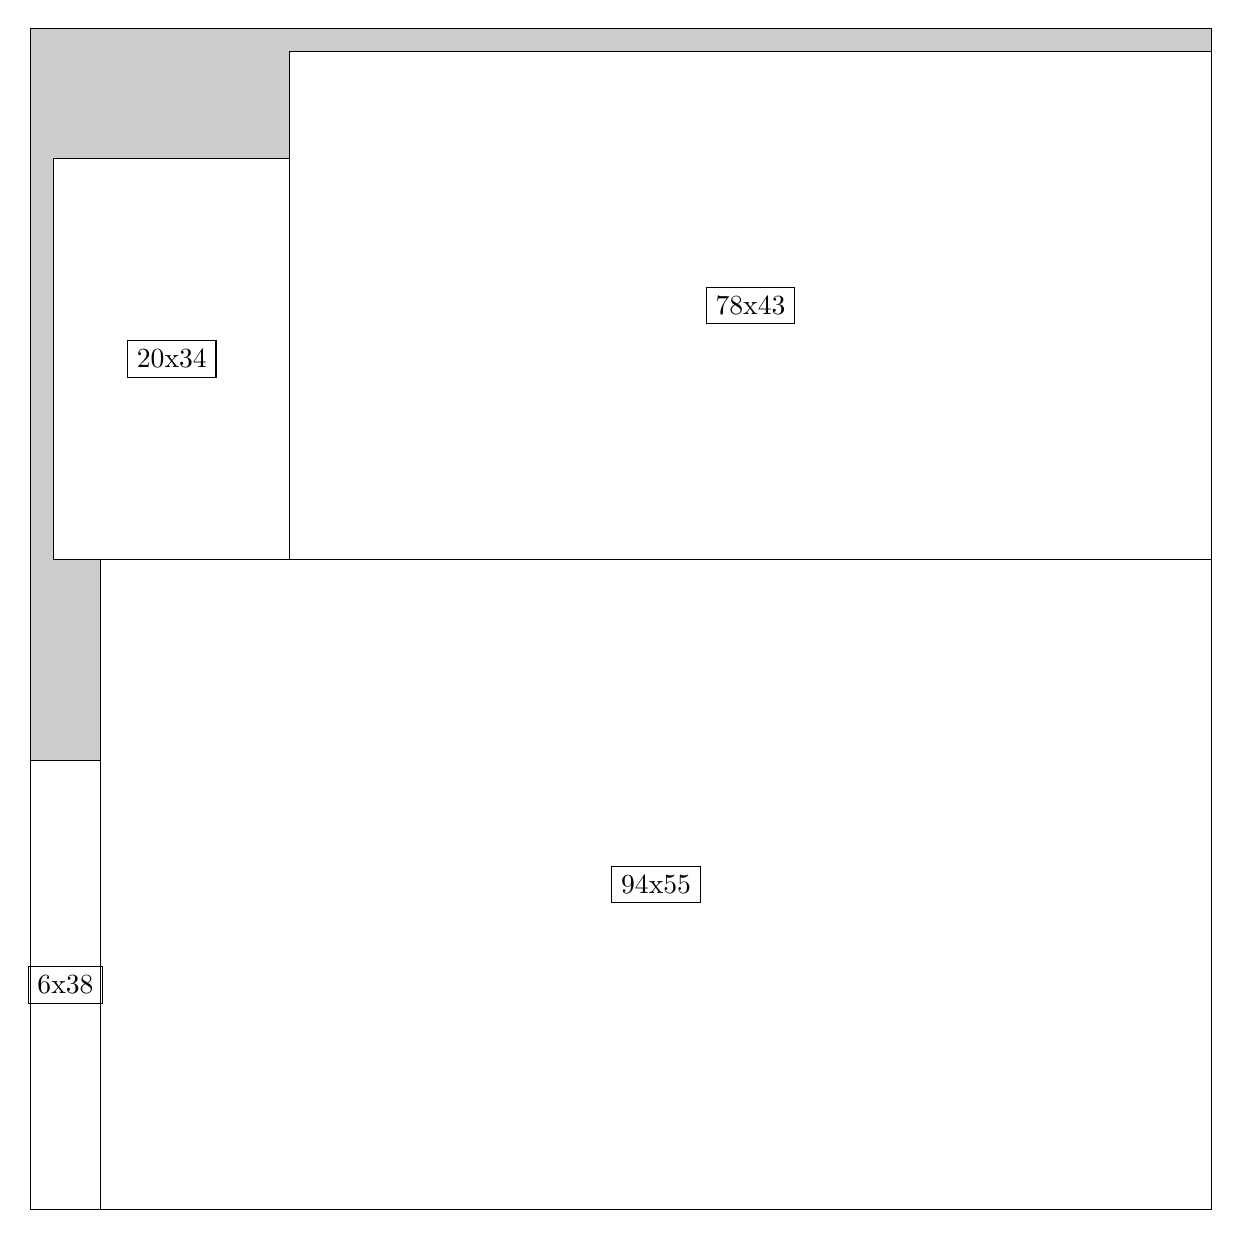
\begin{tikzpicture}[shorten >=1pt,scale=1.0,every node/.style={scale=1.0},->]
\tikzstyle{vertex}=[circle,fill=black!25,minimum size=14pt,inner sep=0pt]
\filldraw[fill=gray!40!white, draw=black] (0,0) rectangle (15.0,15.0);
\foreach \name/\x/\y/\w/\h in {94x55/0.8999999999999999/0.0/14.1/8.25,6x38/0.0/0.0/0.8999999999999999/5.7,78x43/3.3/8.25/11.7/6.45,20x34/0.3/8.25/3.0/5.1}
\filldraw[fill=white!40!white, draw=black] (\x,\y) rectangle node[draw] (\name) {\name} ++(\w,\h);
\end{tikzpicture}


w =94 , h =55 , x =6 , y =0 , v =5170
\par
w =6 , h =38 , x =0 , y =0 , v =228
\par
w =78 , h =43 , x =22 , y =55 , v =3354
\par
w =20 , h =34 , x =2 , y =55 , v =680
\par
\newpage


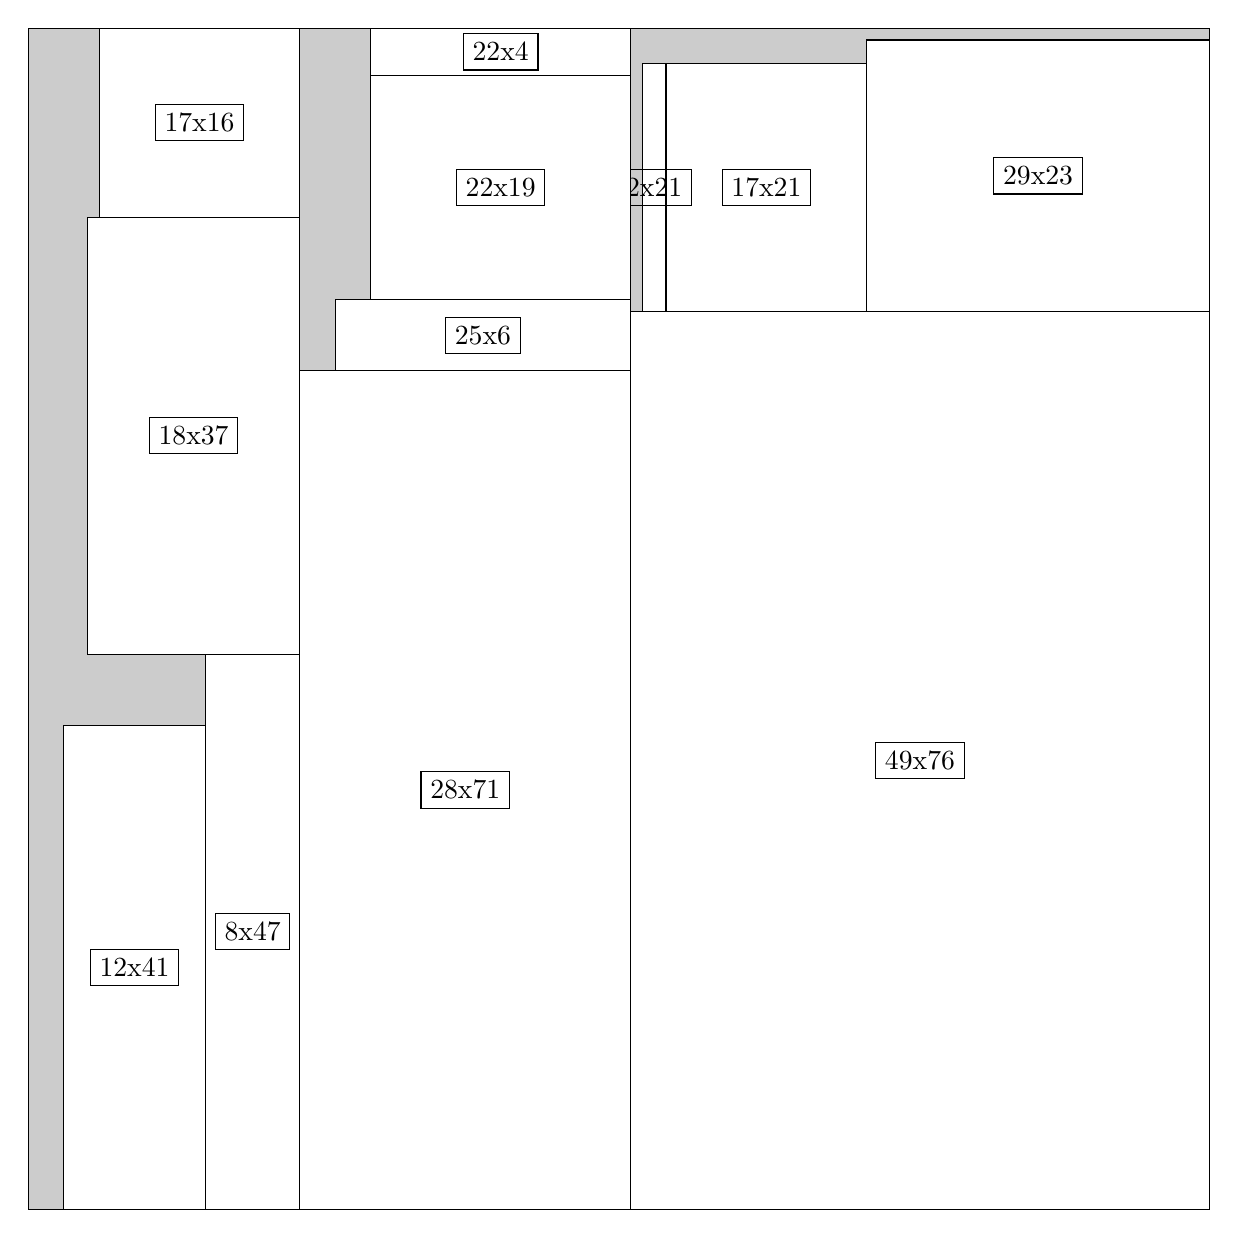
\begin{tikzpicture}[shorten >=1pt,scale=1.0,every node/.style={scale=1.0},->]
\tikzstyle{vertex}=[circle,fill=black!25,minimum size=14pt,inner sep=0pt]
\filldraw[fill=gray!40!white, draw=black] (0,0) rectangle (15.0,15.0);
\foreach \name/\x/\y/\w/\h in {49x76/7.6499999999999995/0.0/7.35/11.4,29x23/10.65/11.4/4.35/3.4499999999999997,17x21/8.1/11.4/2.55/3.15,2x21/7.8/11.4/0.3/3.15,28x71/3.4499999999999997/0.0/4.2/10.65,25x6/3.9/10.65/3.75/0.8999999999999999,22x19/4.35/11.549999999999999/3.3/2.85,22x4/4.35/14.399999999999999/3.3/0.6,8x47/2.25/0.0/1.2/7.05,12x41/0.44999999999999996/0.0/1.7999999999999998/6.1499999999999995,18x37/0.75/7.05/2.6999999999999997/5.55,17x16/0.8999999999999999/12.6/2.55/2.4}
\filldraw[fill=white!40!white, draw=black] (\x,\y) rectangle node[draw] (\name) {\name} ++(\w,\h);
\end{tikzpicture}


w =49 , h =76 , x =51 , y =0 , v =3724
\par
w =29 , h =23 , x =71 , y =76 , v =667
\par
w =17 , h =21 , x =54 , y =76 , v =357
\par
w =2 , h =21 , x =52 , y =76 , v =42
\par
w =28 , h =71 , x =23 , y =0 , v =1988
\par
w =25 , h =6 , x =26 , y =71 , v =150
\par
w =22 , h =19 , x =29 , y =77 , v =418
\par
w =22 , h =4 , x =29 , y =96 , v =88
\par
w =8 , h =47 , x =15 , y =0 , v =376
\par
w =12 , h =41 , x =3 , y =0 , v =492
\par
w =18 , h =37 , x =5 , y =47 , v =666
\par
w =17 , h =16 , x =6 , y =84 , v =272
\par
\newpage


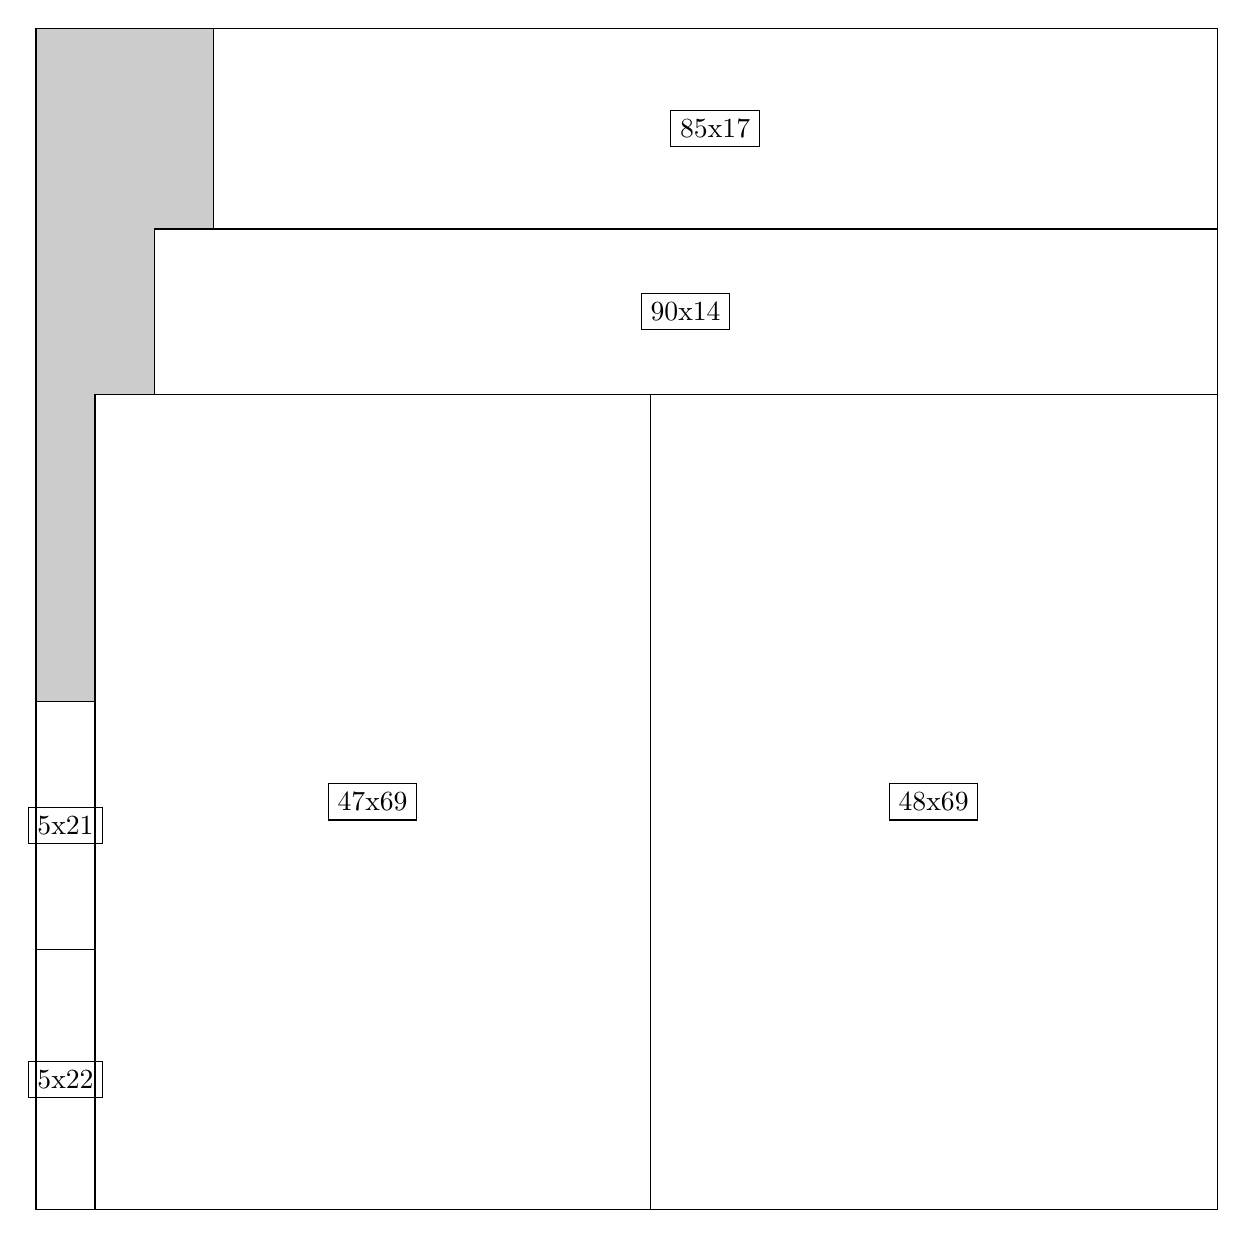
\begin{tikzpicture}[shorten >=1pt,scale=1.0,every node/.style={scale=1.0},->]
\tikzstyle{vertex}=[circle,fill=black!25,minimum size=14pt,inner sep=0pt]
\filldraw[fill=gray!40!white, draw=black] (0,0) rectangle (15.0,15.0);
\foreach \name/\x/\y/\w/\h in {48x69/7.8/0.0/7.199999999999999/10.35,47x69/0.75/0.0/7.05/10.35,5x22/0.0/0.0/0.75/3.3,5x21/0.0/3.3/0.75/3.15,90x14/1.5/10.35/13.5/2.1,85x17/2.25/12.45/12.75/2.55}
\filldraw[fill=white!40!white, draw=black] (\x,\y) rectangle node[draw] (\name) {\name} ++(\w,\h);
\end{tikzpicture}


w =48 , h =69 , x =52 , y =0 , v =3312
\par
w =47 , h =69 , x =5 , y =0 , v =3243
\par
w =5 , h =22 , x =0 , y =0 , v =110
\par
w =5 , h =21 , x =0 , y =22 , v =105
\par
w =90 , h =14 , x =10 , y =69 , v =1260
\par
w =85 , h =17 , x =15 , y =83 , v =1445
\par
\newpage


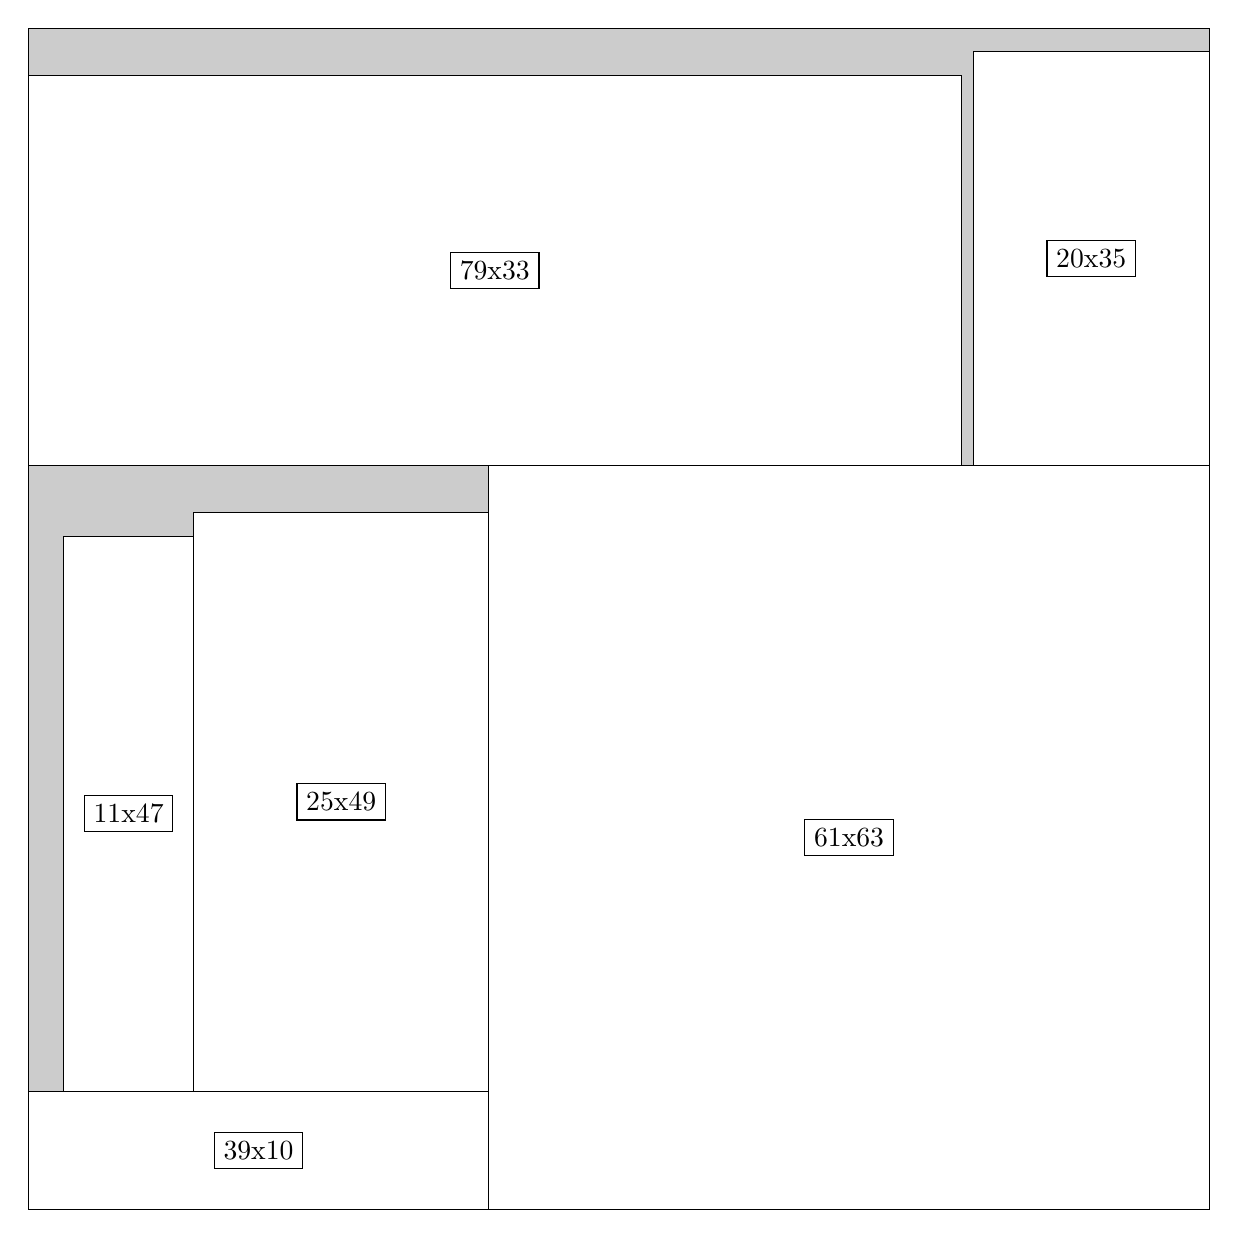
\begin{tikzpicture}[shorten >=1pt,scale=1.0,every node/.style={scale=1.0},->]
\tikzstyle{vertex}=[circle,fill=black!25,minimum size=14pt,inner sep=0pt]
\filldraw[fill=gray!40!white, draw=black] (0,0) rectangle (15.0,15.0);
\foreach \name/\x/\y/\w/\h in {61x63/5.85/0.0/9.15/9.45,39x10/0.0/0.0/5.85/1.5,25x49/2.1/1.5/3.75/7.35,11x47/0.44999999999999996/1.5/1.65/7.05,20x35/12.0/9.45/3.0/5.25,79x33/0.0/9.45/11.85/4.95}
\filldraw[fill=white!40!white, draw=black] (\x,\y) rectangle node[draw] (\name) {\name} ++(\w,\h);
\end{tikzpicture}


w =61 , h =63 , x =39 , y =0 , v =3843
\par
w =39 , h =10 , x =0 , y =0 , v =390
\par
w =25 , h =49 , x =14 , y =10 , v =1225
\par
w =11 , h =47 , x =3 , y =10 , v =517
\par
w =20 , h =35 , x =80 , y =63 , v =700
\par
w =79 , h =33 , x =0 , y =63 , v =2607
\par
\newpage


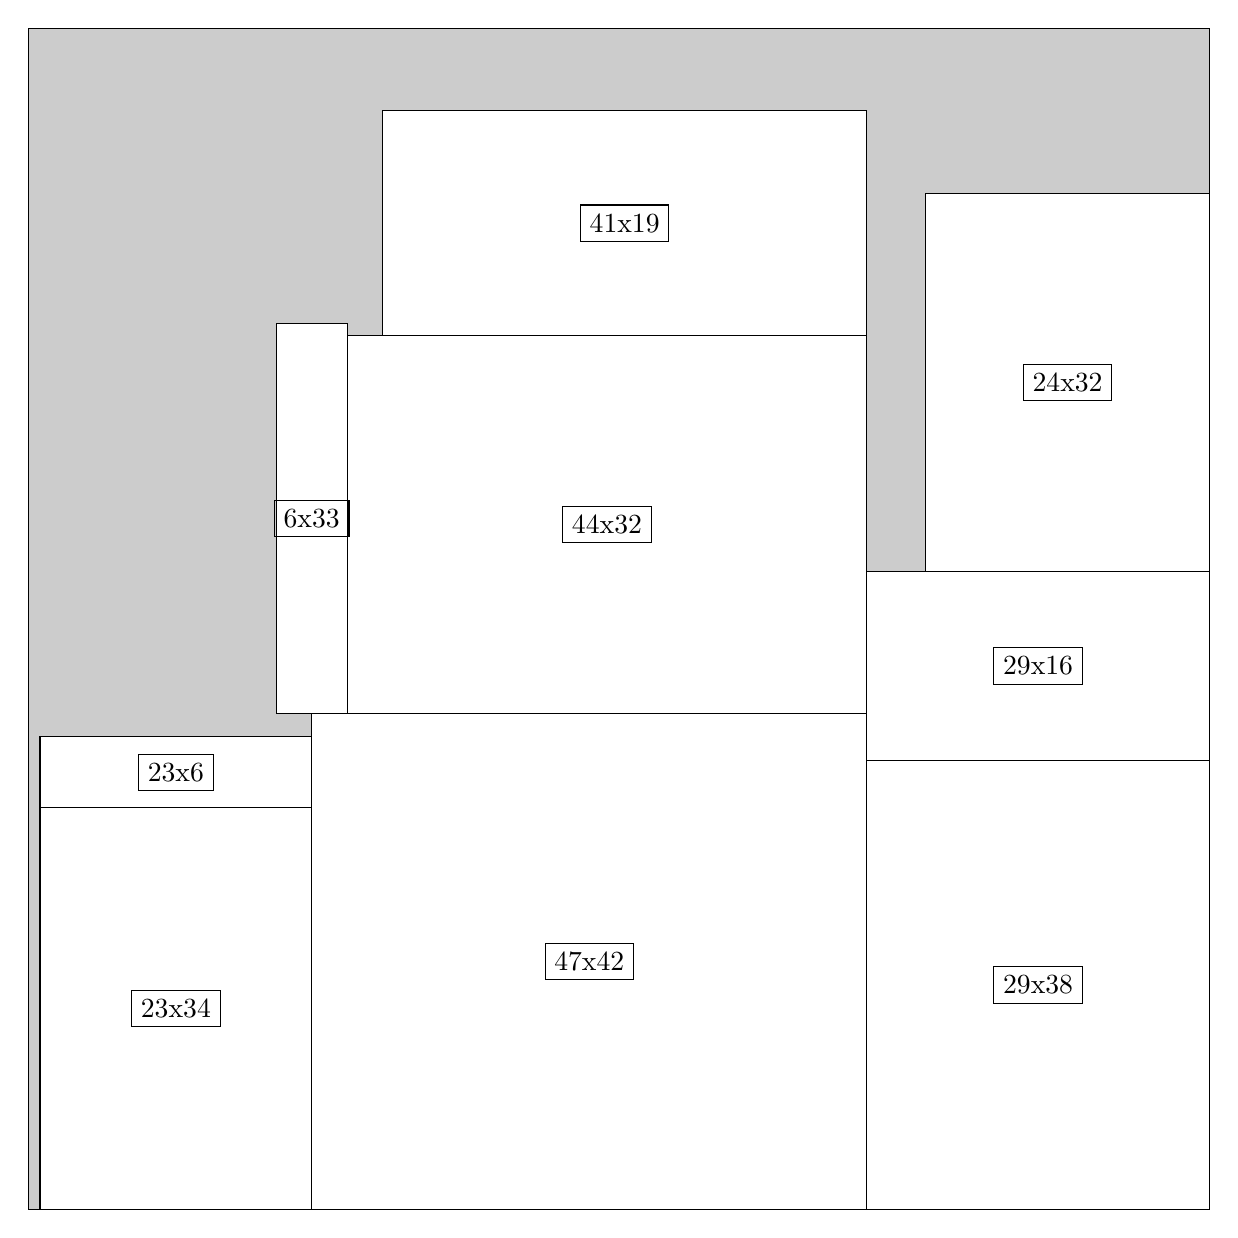
\begin{tikzpicture}[shorten >=1pt,scale=1.0,every node/.style={scale=1.0},->]
\tikzstyle{vertex}=[circle,fill=black!25,minimum size=14pt,inner sep=0pt]
\filldraw[fill=gray!40!white, draw=black] (0,0) rectangle (15.0,15.0);
\foreach \name/\x/\y/\w/\h in {29x38/10.65/0.0/4.35/5.7,29x16/10.65/5.7/4.35/2.4,24x32/11.4/8.1/3.5999999999999996/4.8,47x42/3.5999999999999996/0.0/7.05/6.3,23x34/0.15/0.0/3.4499999999999997/5.1,23x6/0.15/5.1/3.4499999999999997/0.8999999999999999,44x32/4.05/6.3/6.6/4.8,41x19/4.5/11.1/6.1499999999999995/2.85,6x33/3.15/6.3/0.8999999999999999/4.95}
\filldraw[fill=white!40!white, draw=black] (\x,\y) rectangle node[draw] (\name) {\name} ++(\w,\h);
\end{tikzpicture}


w =29 , h =38 , x =71 , y =0 , v =1102
\par
w =29 , h =16 , x =71 , y =38 , v =464
\par
w =24 , h =32 , x =76 , y =54 , v =768
\par
w =47 , h =42 , x =24 , y =0 , v =1974
\par
w =23 , h =34 , x =1 , y =0 , v =782
\par
w =23 , h =6 , x =1 , y =34 , v =138
\par
w =44 , h =32 , x =27 , y =42 , v =1408
\par
w =41 , h =19 , x =30 , y =74 , v =779
\par
w =6 , h =33 , x =21 , y =42 , v =198
\par
\newpage


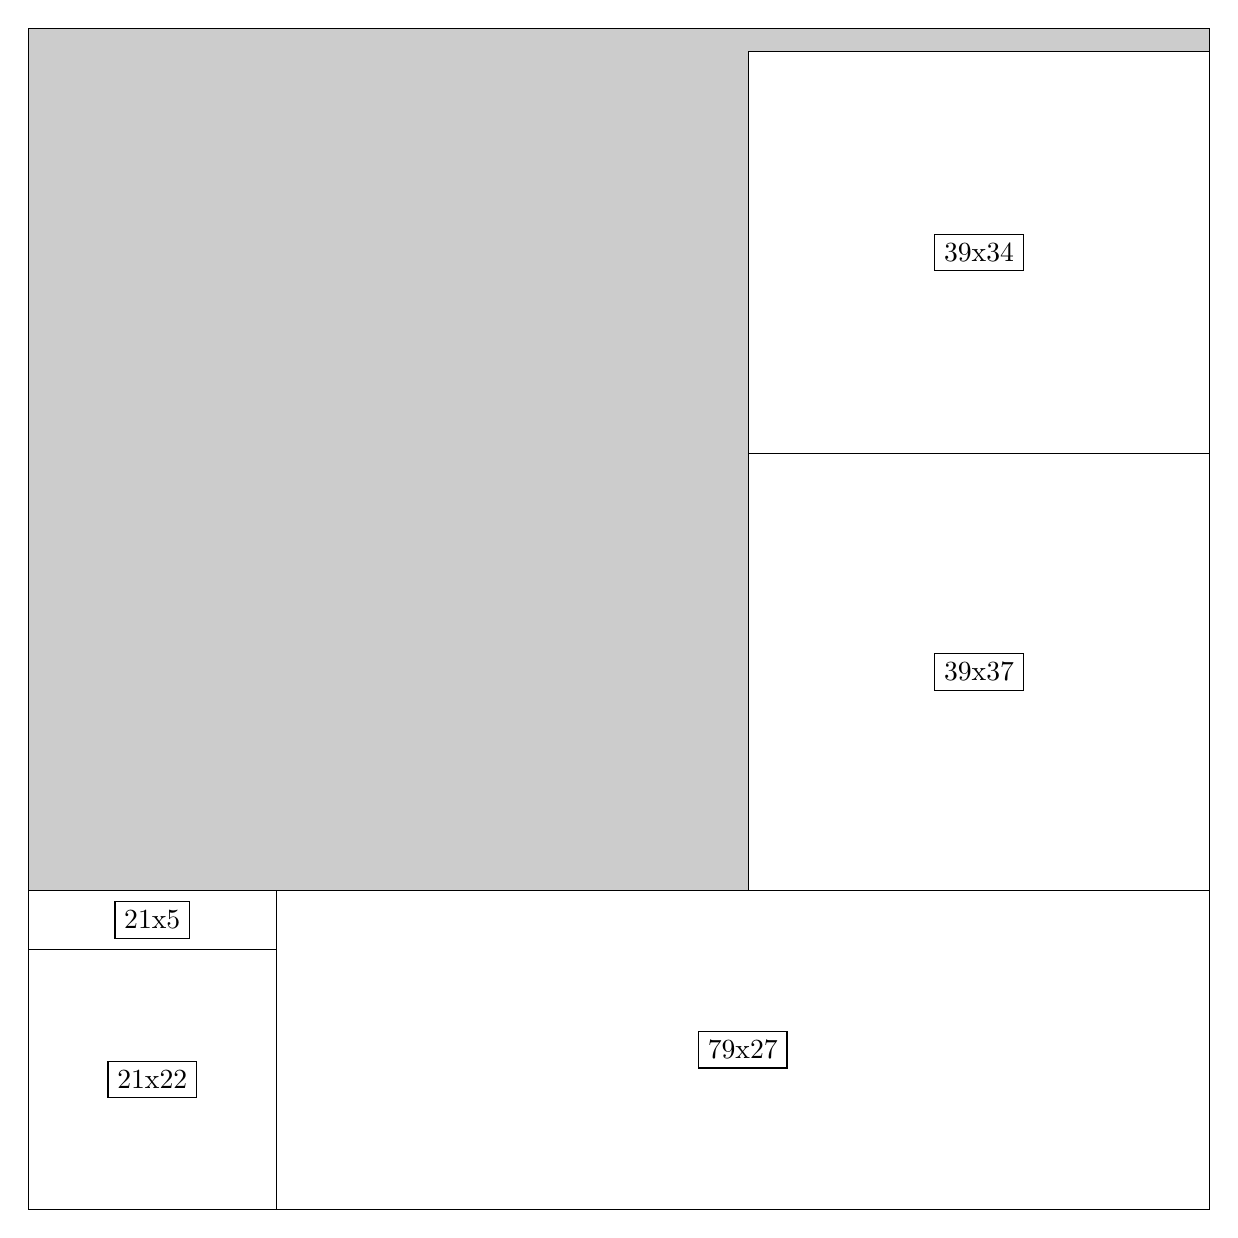
\begin{tikzpicture}[shorten >=1pt,scale=1.0,every node/.style={scale=1.0},->]
\tikzstyle{vertex}=[circle,fill=black!25,minimum size=14pt,inner sep=0pt]
\filldraw[fill=gray!40!white, draw=black] (0,0) rectangle (15.0,15.0);
\foreach \name/\x/\y/\w/\h in {79x27/3.15/0.0/11.85/4.05,21x22/0.0/0.0/3.15/3.3,21x5/0.0/3.3/3.15/0.75,39x37/9.15/4.05/5.85/5.55,39x34/9.15/9.6/5.85/5.1}
\filldraw[fill=white!40!white, draw=black] (\x,\y) rectangle node[draw] (\name) {\name} ++(\w,\h);
\end{tikzpicture}


w =79 , h =27 , x =21 , y =0 , v =2133
\par
w =21 , h =22 , x =0 , y =0 , v =462
\par
w =21 , h =5 , x =0 , y =22 , v =105
\par
w =39 , h =37 , x =61 , y =27 , v =1443
\par
w =39 , h =34 , x =61 , y =64 , v =1326
\par
\newpage


\end{document}